\documentclass[12pt,a4paper]{report}

\usepackage[utf8]{inputenc} % un package
\usepackage[T1]{fontenc}      % un second package
\usepackage[francais]{babel}  % un troisième package
\usepackage[top=2cm, bottom=2cm, left=2cm, right=2cm]{geometry}
\usepackage{titlesec} 
\usepackage{graphicx}
\usepackage{caption}
\captionsetup{figurewithin=none}  
\captionsetup{tablewithin=none}
\makeatletter
\usepackage{listings}
\usepackage{color}
 
\definecolor{dkgreen}{rgb}{0,0.6,0}
\definecolor{mauve}{rgb}{0.58,0,0.82}
 
\lstset{ %
	language=sh,                % the language of the code
  basicstyle=\footnotesize,           % the size of the fonts that are used for the code
  numbers=left,                   % where to put the line-numbers
  numberstyle=\footnotesize,          % the size of the fonts that are used for the line-numbers
  stepnumber=1,                   % the step between two line-numbers. If it's 1, each line 
                                  % will be numbered
  numbersep=5pt,                  % how far the line-numbers are from the code
  backgroundcolor=\color{white},      % choose the background color. You must add \usepackage{color}
  showspaces=false,               % show spaces adding particular underscores
  showstringspaces=false,         % underline spaces within strings
  showtabs=false,                 % show tabs within strings adding particular underscores
  frame=single,                   % adds a frame around the code
  tabsize=2,                      % sets default tabsize to 2 spaces
  captionpos=b,                   % sets the caption-position to bottom
  breaklines=true,                % sets automatic line breaking
  breakatwhitespace=false,        % sets if automatic breaks should only happen at whitespace
  title=\lstname,                   % show the filename of files included with \lstinputlisting;
                                  % also try caption instead of title
  numberstyle=\tiny\color{red},        % line number style
  keywordstyle=\color{blue},          % keyword style
  commentstyle=\color{dkgreen},       % comment style
  stringstyle=\color{mauve},         % string literal style
  escapeinside={\%*}{*)},            % if you want to add a comment within your code
  morekeywords={mkdir,hg}               % if you want to add more keywords to the set
}
\def\clap#1{\hbox to 0pt{\hss #1\hss}}%
\def\ligne#1{%
\hbox to \hsize{%
\vbox{\centering #1}}}%
\def\haut#1#2#3{%
\hbox to \hsize{%
\rlap{\vtop{\raggedright #1}}%
\hss
\clap{\vtop{\centering #2}}%
\hss
\llap{\vtop{\raggedleft #3}}}}%
\def\bas#1#2#3{%
\hbox to \hsize{%
\rlap{\vbox{\raggedright #1}}%
\hss
\clap{\vbox{\centering #2}}%
\hss
\llap{\vbox{\raggedleft #3}}}}%
\def\maketitle{%
\thispagestyle{empty}\vbox to \vsize{%
\haut{}{\@blurb}{}
\vfill
\vspace{1cm}
\begin{flushleft}
\usefont{OT1}{ptm}{m}{n}
\huge \@title
\end{flushleft}
\par
\hrule height 4pt
\par
\begin{flushright}
\usefont{OT1}{phv}{m}{n}
\Large \@author
\par
\end{flushright}
\vspace{1cm}
\vfill
\vfill
\bas{}{{\textbf{\Large Responsable : Mme. THEBAULT\\ \textbf{} \\ \@location, le \@date}}}{}
}%
\cleardoublepage
}
\def\date#1{\def\@date{#1}}
\def\author#1{\def\@author{#1}}
\def\title#1{\def\@title{#1}}
\def\location#1{\def\@location{#1}}
\def\blurb#1{\def\@blurb{#1}}
%%%%%%%%%%%%%%%%%%%%%%%%%%%%%%%%%%%%%%%%%%%%%%%
%% Informations relatives au projet en cours %%
%%%%%%%%%%%%%%%%%%%%%%%%%%%%%%%%%%%%%%%%%%%%%%%

\date{30 Janvier 2012}
\author{}
\title{}
\location{Bordeaux}\blurb{}
\makeatother
\title{Analyse technique de logiciel\\Galaxy}
\author{Florian CARRE\\Benjamin DARTIGUES\\Sebastien BEAUQUIS\\Guillaume BERNARD\\Tom LESLUYES}
\location{Bordeaux}
\blurb{%
\begin{Large}
\textbf{Université Bordeaux 1\\Master 2 Bioinformatique}
\end{Large} \\

\includegraphics[scale=0.7]{bdx1.png}
\graphicspath{img/} %% Chemin vers les images du projets
}
\titleformat{\chapter}[hang]{\bf\huge}{\thechapter}{2pc}{} 
\titleformat{\part}[hang]{\bf\huge}{\thepart}{2pc}{} 


%%%%%%%%%%%%%%%%%%%%%%%%%
%% Contenu du document %%
%%%%%%%%%%%%%%%%%%%%%%%%%

\begin{document}

\maketitle  %% Création de la page de guarde
\tableofcontents  %% Création d'une table des matière
\thispagestyle{empty}
\newpage\pagenumbering{arabic}
%\thispagestyle{fancy}


%%%%%%%%%%%%%%%%%%%%%%%%%%%%%%%%%
%% Insertion du corps du texte %%
%%%%%%%%%%%%%%%%%%%%%%%%%%%%%%%%%
\chapter*{Introduction}
\addcontentsline{toc}{chapter}{Introduction}

Le séquençage du génome, c'est à dire l'ensemble du code ADN d'un être vivant, s'est transformé ces dernières années en une course effrénée entre laboratoires concurrents.\\

Cette course a contribué à l'explosion de la quantité de données à traiter, données fournies par les séquenceurs nouvelle génération. L'étude de ces données nécessite de posséder des outils de grande fiabilité mais surtout possédant un large panel de traitements applicables à ses mêmes données.\\

 En effet, étudier le génome ne se limite pas à un simple déchiffrage du code contenu dans l'ADN, l'objectif reste principalement de comprendre le génome en analysant les gènes et les régions intergéniques, en évaluant le niveau d'expression de gènes par rapport à d'autres, en comparant les génomes de différentes espèces entre eux afin d'en sortir des lois et des règles.\\
 
 Il existe de nombreuses plates formes sur le web ainsi que de nombreux logiciels dédiés à l'étude des données issues du séquençage. Notre regard s'est porté sur Galaxy\footnote{\cite{afgan2010galaxy}\cite{afgan2011harnessing}\cite{afganreference}\cite{afgan2011galaxy}\cite{blankenberg2011integrating}\cite{blankenberg2010manipulation}\cite{blankenberg2011making}\cite{blankenberg2007framework}\cite{bock2010web}\cite{giardine2005galaxy}\cite{goecks2011galaxy}\cite{lazarus2008toward}\cite{miller200728}\cite{pond2009windshield}\cite{schatz2010missing}}, à la fois une plate forme web et un logiciel open source, qui présente une multitude de traitements à appliquer aux données du génome.\\
 
 Nous présenterons ainsi une revue sommaire des logiciels existants à ce jour puis nous vous exposerons une série de traitements réalisés afin de mettre en exergue les qualités et les défauts inhérents à ce logiciel.

\chapter{Présentation}

\section{État de l'art}

nous présentons ici une revue des principaux logiciels "concurrents" ou du moins répondant aux mêmes types de problématiques que Galaxy. Certains parmi eux ne réalisent qu'une petite partie des traitements accomplis par Galaxy. Quant aux autres, rares sont ceux qui offrent autant de liberté et de facilité d'utilisation. De plus, la plupart sont payants et offre donc seulement des versions d'essais limités.

\subsection{CLC bio genomics workbench }
\subsubsection{Description}
c'est une plate forme commerciale et une extension du logiciel CLCbio Main Workbench .
On peut uniquement obtenir une version d'essai pour 15 jours.
\begin{itemize}
\item{assembleur de séquences de novo (inclus la détection des sNP , CHiP-seq).}
\item{Composition du génome }
\item{Analyse des séquences (gènes et régions intergéniques)}
\item{Nombre de gènes et leur position sur les chromosomes }
\item{Niveau d’expression des gènes }
\item{Comparaison des génomes de diverses espèces (génomique comparative)}
\end{itemize}
\subsubsection{Système d'exploitation}
 Windows, Mac OS X et Linux.
\subsection{Genomatix}
\subsubsection{Description}
Genomatix propose des solutions et des services pour l'ensemble du déroulement de l'analyse, de la cartographie de premier niveau à l'intégration des résultats multiples avec des copies des fond des données de haute qualité. Les technologies de visualisation et d'interprétation permettent aux scientifiques du monde entier de transformer leurs données en résultats significatifs, transformant le séquençage nouvelle génération en un outil parfait appliqué à la médecine personnalisée. Il se décompose en trois grandes entités que sont Genomatix Genome Analyzer (GGA), Genomatix Station  mining (GMS) et Genomatix Software Suite.
\subsubsection{Genomatix Genome Analyzer (GGA)}
Genomatix Genome Analyzer (GGA) est une solution intégrée complète pour la visualisation et l'interprétation de Next Generation Sequencing (NGS) de données de la puce à ARN,d'ADN,ou de petit séquençage d'ARN. Chaque analyseur est pourvu d'un état de l'art des technologies ce qui éclaire le contexte biologique. Le GGA produit des résultats de grande pertinence. Les données de base biologiques comprenant des données du réseau d'annotation et de gènes fournis par Eldorado, ainsi que la connaissance des facteurs de transcription contenues dans MatBase permettent aux chercheurs d'analyser et d'interpréter leurs résultats expérimentaux dans un contexte biologique unique sur chaque GGA et sur plus de 30 espèces différentes. L'analyse de l'expression différentielle (jusqu'au niveau de transcription), la vérification du réseau, l' analyse de la littérature ne sont que quelques-unes des tâches qui peuvent être effectuées.
\subsubsection{Genomatix Station mining (GMS)}
Genomatix Station Mining (GMS) offre un alignement haute performance des séquençages de nouvelle génération (NGS). 
Elle permet de lire sur les génomes, transcriptomes, petit ARN. Avec son interface utilisateur intuitive, le GMS vous aide à exécuter rapidement des tâches telles que le positionnement génomique, SNP et détection d'Indel, des analyses d'épissage, la fusion de gènes et l'analyse structurelle. De plus, la station reste souple tout au long de l'expérience. En combinaison avec le Genome Analyzer Genomatix on obtient une solution d'analyse entièrement intégrée à partir du séquençage et pratique pour l'interprétation
\subsubsection{Genomatix Software Suite}
Un bundle de logiciels bien établis, la suite logicielle Genomatix effectue un certain nombre de tâches:
\begin{itemize}
\item{Elle procède à une analyse scientifique des données génomiques, la régulation des gènes et l'expression}
\item{Elle génère et évalue les réseaux et les voies}
\item{Elle effectue des recherches documentaires étendues et des analyses de séquence et de l'extraction}
\item{Elle visualise les annotations des génomes complets.}
\end{itemize}

\subsection{Ergatis}
\subsubsection{Description}

Ergatis est un utilitaire-Web  utilisé pour créer, exécuter et contrôler les pipelines réutilisables en analyse informatique. Elle contient des composants pré-construits pour les tâches courantes d'analyse bioinformatique. Ces composants peuvent être disposées graphiquement pour former des pipelines hautement configurables . Chaque composant d'analyse soutient plusieurs formats de sortie, y compris la séquence Bioinformatic Markup Language (BSML). L'implémentation actuelle inclut le support pour le chargement des données dans des bases de projet suivant le schéma Chado, un schéma normalisé soutenue par la communauté  pour le stockage des données biologiques.

Ergatis utilise le moteur de workflow pour traiter ses travaux sur une grille de calcul. Workflow fournit un langage XML et du moteur de traitement pour préciser les étapes d'un pipeline de calcul. Il fournit l'état d'exécution détaillé, facilite la récupération d'erreur au point de défaillance, et est hautement évolutive avec un support pour les environnements informatiques les plus distribués. Le format XML utilisé permet d'exécuter les commandes  en série, en parallèle, et dans n'importe quelle combinaison ou niveau d'imbrication.

Ce cadre de travail a été employé dans l'annotation de plusieurs grands organismes eucaryotes, y compris Aedes aegypti et Trichomonas vaginalis.
Ce projet est à ce jour fonctionnel tout en étant en cours de développement actif, avec la plupart des codes proviennent de contribution avec l'Institut des sciences du génome et le J. Craig Venter Institute.


\subsection{JMP Genomics}
\subsubsection{Description}
JMP Genomics est un logiciel de découverte statistique issu de deux références dans les logiciels analytiques: SAS et JMP. Les organismes de recherche utilisent JMP Genomics pour découvrir des modes significatifs dans la génétique à haut débit, l'expression des génes, le nombre de copies et les données protéomiques. l'Interaction graphique dynamique rend facile à explorer les données en relation avec un ensemble complet d' algorithmes avancés de statistiques.

\subsubsection{Système d'exploitation}
on trouve une version 9 qui est compatible avec Windows et Mac. Les versions antérieures sont quand à elles compatibles aussi avec Linux.

\subsection{Lasergene 9.1}
\subsubsection{Description}
Lasergene 9.1 comprend de nouveaux assembleurs de séquences "next-gen", des workflows d'analyse et les séquences, structures et vues d'analyse des protéines intégrées. Cela fait  vraiment de Lasergene un des logiciels  intégrés les plus fiables du marché soutenant l'analyse de séquence traditionnelle, l'assemblage de séquences next-gen ainsi que leurs analyses, les études d'expression génique, l'analyse d'ARN-Seq et de ChIP-Seq.
\subsubsection{Système d'exploitation}
Windows, Mac et Linux
\subsection{RTG}
\subsubsection{Description}
L'analyse de séquence avec RTG offre des applications de séquençage de l'adn pour la recherche clinique sur les maladies génétiques et les maladies rares.le logiciel fournit une sensibilité maximale de la  lecture de la cartographie dans l'alignement des séquences nucléotidiques sans sacrifier à la vitesse de traitement .
\subsubsection{Système d'exploitation}

\subsection{life appliedbiosystems}
\subsubsection{Description}





\section{Séquençage nouvelle génération}
\subsection*{Historique}
	Le séquençage de l'ADN a été inventé dans la fin des années 1970.
Deux méthodes ont été développées indépendamment.
L'une, basé sur la \textbf{synthèse enzymatique} sélective et réalisé par l'équipe de Frederick Sanger en Angleterre.
La deuxième, basé sur la \textbf{dégradation chimique} sélective a été réalisée par l'équipe de Walter Gilbert aux États-Unis.
Tout deux ont été récompensé du prix Nobel de chimie pour cette découverte en 1980.

~~\\
La technique de séquençage de Walter Gilbert était le prémisse du pyroséquençage. Cette technique est principalement basé sur l'addition d'un seul nucléotide qui est révélé en temps réel par détection de la  luminescence. 
~~\\
Au début du XXème siècle, de nouvelles techniques de séquençage couplées aux connaissances en physique, chimie, informatique, nanotechnologie et biotechnologie ont vu le jour, et permettent d'augmenter le débit du séquençage par une parallélisation massive des réactions et par miniaturisation des supports utilisés.
~~\\
Nous allons décrire deux plateformes de séquençage novatrices qui, aujourd'hui encore, sont les modèles en matière de séquençage haut-débit.
~~\\
\begin{itemize}
\item[$\bullet$]la technologie 454 (le pyroséquençage).
\item[$\bullet$]la technologie Solexa (Illumina).
\end{itemize}
	
\subsection*{Les différents types de séquençage haut-débit{\scriptsize \cite{NGS}\cite{NGS2}\cite{NGS3}\cite{NGS4}\cite{NGS5}}}
	\subsubsection*{Le pyroséquençage}
	~~\\
Le pyroséquençage est donc une version amèliorée de la technique de Maxam et Walter. Il a été élaboré par Hyman et al., un groupe suédois. Le principe est d'utiliser la technique de Walter en l'a couplant avec la technique de PCR (Réaction en Chaine par Polymerase). C'est une technique de séquençage par \textbf{synthèse}.

~~\\
La technique de pyroséquençage réside en X étapes:

~~\\
Premièrement, on réalise une bibliothèque des séquences que l'on veut séquencé (à l'aide d'une séquence de ligation qui va se coupler à la séquence).

~~\\
On extrait la séquence puis on lui fixe une séquence dite adapteur. La séquence adapteur est complémentaire d'une séquence fixée à une micro-bille. On attache donc la séquence d’intérêt à une micro-bille. On dispose de nombreuses micro-billes préparées de la même façon dans des puces à ADN puis on polymérise la séquence par PCR.
~~\\
\begin{figure}[!h]
 \centering
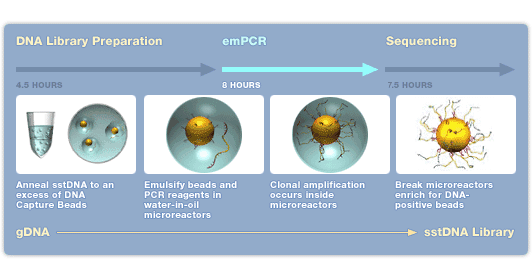
\includegraphics[scale=0.8]{Images/microbille.png}
\caption{Ligation des séquences aux microbilles.}
\end{figure}
\newpage
~~\\
\begin{figure}[!h]
 \centering
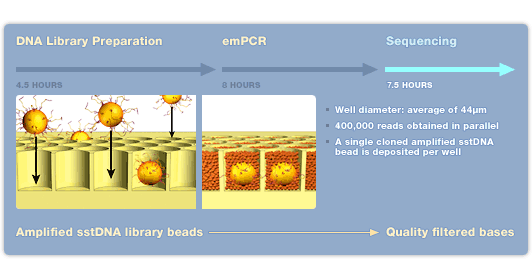
\includegraphics[scale=0.8]{Images/incbil.png}
\caption{Incorporation des billes dans la puce à ADN.}
\end{figure}

On dispose la puce dans une cuve contenant :
~~\\
\begin{itemize}
\item de la Sulfurylase,
\item de la Luciferase,
\item de l'Apyrase,
\item de la Polymerase.
\end{itemize}
~~\\
Le tableau ci-dessous explique le rôle de chacune des enzymes listées précédemment:
~~\\

\begin{tabular}{|c|c|c|c|c|}
	\hline
   Enzymes & Rôles \\
   \hline
   Sulfurylase & Convertie un pyrophosphate en adenosine tri-phosphate (ATP). \\
   \hline
   Luciferase & Emet de la lumière en consommant un ATP. \\
   \hline
   Apyrase & Dégrade les nucléotides. \\
   \hline
   Polymerase & Incorpore un acide nucléique complémentaire à un brin d'ADN \\&en consommant un groupement phosphate d'un ATP.\\
   \hline
\end{tabular}

~~\\
~~\\
Ensuite, on incorpore successivement les acides nucléiques de manière sélective au niveau de la puce.

A chaque incorporation d'acides nucléiques, le résidu attendu par la polymérase est intégré dans la chaine ADN pendant l'élongation et libère un pyrophosphate.

L’ATPsulfurylase vient alors transformer ce Pyrophophate (PPi) en ATP qui est alors utilisé, couplé à une Luciférine, par une Luciférase. On a alors production d’Oxyluciférine et d’un signal lumineux.

L'Apyrase dégrade les acides nucléotidiques en surplus dans le milieu.
~~\\
\newpage
\begin{figure}[!h]
   \begin{minipage}[b]{0.40\linewidth}
      \centering 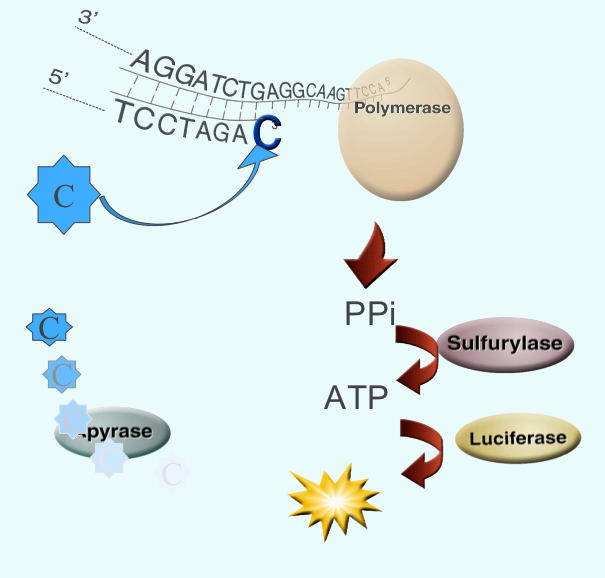
\includegraphics[scale=0.3]{Images/proces.png}
   \end{minipage}\hfill
   \begin{minipage}[b]{0.48\linewidth}   
      \centering 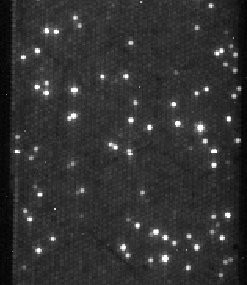
\includegraphics[scale=0.4]{Images/454.png}
   \end{minipage}
   \caption{Représentation des étapes réactionnelles pour obtenir le signal lumineux.}
\end{figure}
~~\\
Le signale lumineux est capté par un capteur CCD (Charge-Coupled Device) puis reproduit sous forme d’un pic sur le Pyrogramme.La hauteur de ce pic est fonction de l'intensité de la lumière, elle-même proportionnelle de la quantité de l'acide nucléique intégré.
\begin{figure}[!h]
   \begin{minipage}[b]{0.40\linewidth}
      \centering 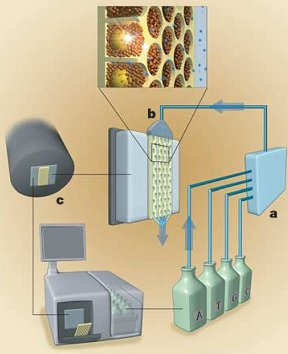
\includegraphics[scale=0.5]{Images/mach.png}
   \end{minipage}\hfill
   \begin{minipage}[b]{0.48\linewidth}   
      \centering 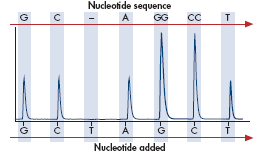
\includegraphics[scale=0.7]{Images/sign.png}
   \end{minipage}
   \caption{Lecture de la séquence à partir des signaux lumineux.}
\end{figure}
\paragraph*{Technique de séquençage Illumina}
~~\\

Illumina est le nom d'un laboratoire développant entre autre le séquençage à partir de la technique de Sanger (la CRT: Cyclic Reversible Termination) ainsi que des connaissances actuelles en biopuces à ADN, nanotechnologies et en informatique de pointe pour l'acquisition, le traitement et l'analyse des images.
~~\\
Cette technique s'applique en plusieurs étapes :
~~\\
\textbf{Étape 1:}
Préparation de la banque d'ADN génomique.
L'ADN génomique est fragmenté par nébulisation. Les extrémités sont réparées et des adaptateurs sont fixés sur chaque extrémité par ligation.
~~\\
\textbf{Étape 2:}
Des ponts d'amplification sont formés sur des plaques ce qui permet d'obtenir de grandes quantités de brins d'ADN, augmentant ainsi le débit de séquençage.
~~\\
\textbf{Étape 3:}
Les brins sont ensuite dénaturés et l'on effectue le séquençage par la technique CRT. 
Les nucléotides fluorescents sont additionnés d'un groupement nitrophenyl en 3'O.
Le nucléotide est incorporé à la séquence lors de la synthèse.
Ensuite, il y a une phase de détection du nucléotide inséré par fluorescence.
L' envoie d'un rayonnement UV (>300nm) détache le groupement nitrophenil de la liaison en 3'O permettant l'incorporation de nouveaux nucléotides.
~~\\
\textbf{Étape 4:}
Interprétation des résultats et lecture de la séquence.
\begin{figure}[!h]
 \centering
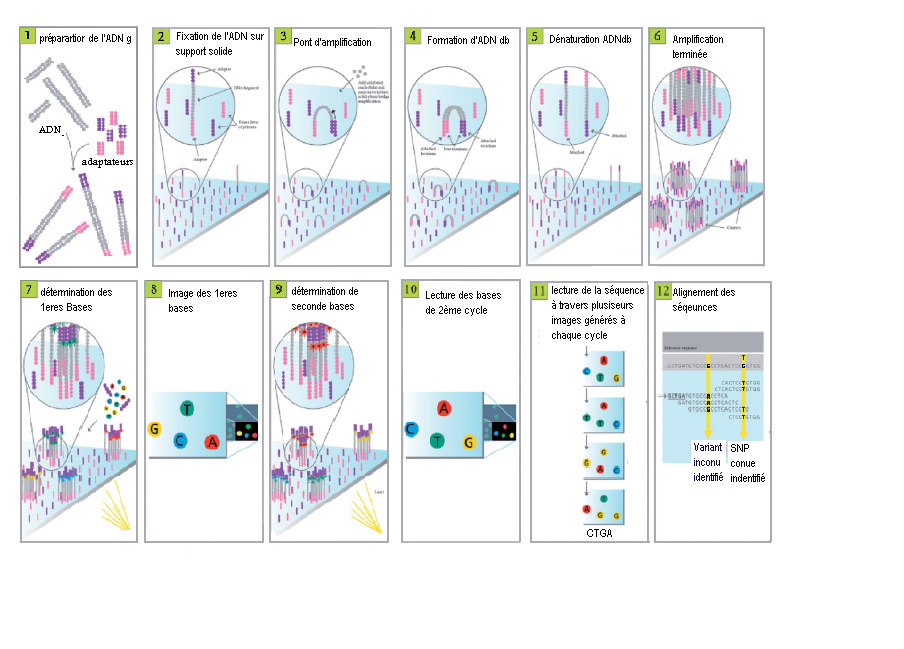
\includegraphics[scale=0.6]{Images/sequfr1.png}
\caption{Différentes étapes de la méthode de séquençage Illumina.}
\end{figure}
~~\\
\chapter{Utilisation}

Galaxy est un logiciel qui peut être utilisé de trois façon différentes : 

\begin{itemize}
\item en ligne, depuis le site web de ce dernier,
\item sur un "cloud",
\item en local, directement sur son ordinateur.\\
\end{itemize}

La création de sa propre instance de Galaxy sur le "cloud" permet une utilisation de celui-ci similaire à celle en local sans l'inconvénient de la place prise en mémoire sur son ordinateur, toutefois un compte Amazon Web Services est requis.\\

La création du compte est gratuite, cependant un numéro de carte bleue doit être renseigné, en effet il semble que l'utilisation de l'ensemble des fonctionnalitées du "cloud" ai un coût. Nous n'avons donc pas pu tester Galaxy sur le "cloud".\\

\section{En ligne}

L'utilisation en ligne de Galaxy est le moyen le plus rapide et le plus accessible : en effet il suffit de se rendre sur le site de ce dernier pour pouvoir y avoir directement accès. Si une utilisation sommaire ne nécessite pas la création d'un compte, il est fortement recommandé d'en créer un (gratuitement) pour avoir accès à plus de fonctionnalité. Posséder un compte sur Galaxy permet :\\

\begin{itemize}
\item d'avoir accès aux données et aux outils d'analyse depuis n'importe quel ordinateur connecté à Internet,
\item augmenter les données et les travaux simultanés,
\item sauvegarder un historique de compte sur une base systémique,
\item d'avoir la capacité de nommer, sauvegarder, partager et publier des objets de Galaxy : des historiques, des workflows, des ensembles de données, des pages.
\item de télécharger via le FTP de plus grands ensembles de données.\\
\end{itemize}

Galaxy dispose de nombreux outils (plus de 35 différents), heureusement lorsque l'on sélectionne l'un d'entre eux une petite fenêtre explicative nous renseigne directement sur ce qu'il fait, le format de données qu'il accepte et un exemple est également proposé (Fig. 6).\\


\begin{figure}[!h]
 \centering
\fbox{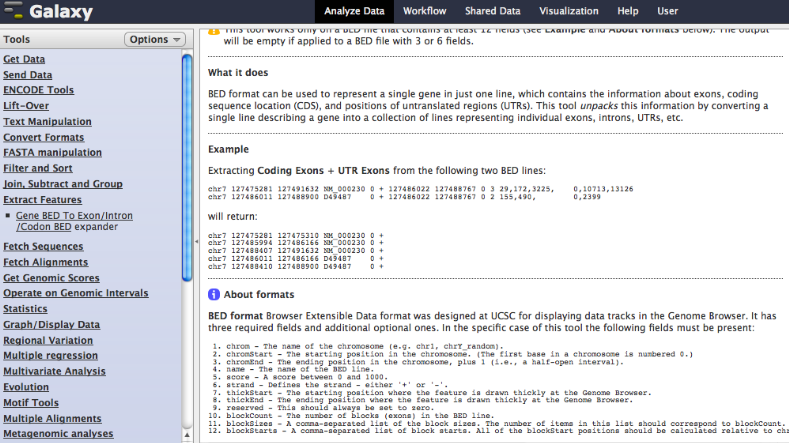
\includegraphics[scale=0.5]{Images/exinfo.png}}
\caption{Page d'aide d'un des outils de Galaxy.}
\end{figure}

Un wiki dédié à Galaxy est disponible sur son site, plusieurs sections différentes permettent d'en apprendre plus sur les données que peut utiliser Galaxy et les outils qu'il propose. De plus de nombreuse vidéos "tutoriel" sont disponibles, ainsi un exercice nommé Galaxy 101 fait office de "tutoriel" de départ et permet de se familiarisé avec le logiciel et quelques unes de ces fonctionnalitées. Une vidéo "tutoriel" est disponible pour chaque outil intégré à Galaxy (Fig. 7).

\begin{figure}[!h]
 \centering
\fbox{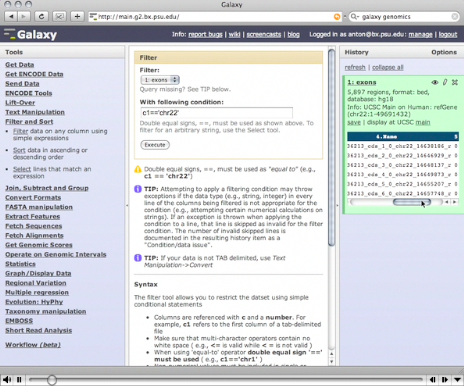
\includegraphics[scale=0.5]{Images/tuto.png}}
\caption{Vidéo "tutoriel" de Galaxy.}
\end{figure}

\section{En local}

En plus de proposer une utilisation via internet, il est possible d'installer Galaxy sur un ordinateur. L'utilisateur peut ainsi profiter de toutes les fonctionnalités de Galaxy et même les personnaliser en vue d'une utilisation spécifique\footnote{Le tutorial officiel de l'installation locale est disponnible à l'adresse suivante :\\ http://wiki.g2.bx.psu.edu/Admin/Get\%20Galaxy}.\\

Par rapport à l'utilisation en ligne, le local présente plusieurs avantages :
\begin{itemize}
\item modifier les paramètres des plug-ins déjà implémentés,
\item ajouter ses propres plug-ins,
\item augmenter la vitesse d'analyse,
\item conserver des données sensibles.\\
\end{itemize}

L'installation est très simple et se déroule en deux étapes :
\begin{enumerate}
\item téléchargement du code source,
\item exécution du serveur local.
\end{enumerate}

\subsection{Téléchargement du code source}

La dernière version stable de Galaxy est toujours disponible depuis un répertoire Mercurial\footnote{http://mercurial.selenic.com/} hébergé sous Bitbucket\footnote{https://bitbucket.org/}. Il existe deux façons de récupérer le code source : en utilisant les outils proposés par Bitbucket ou en utilisant Mercurial.

\subsection*{Bitbucket}

Bitbucket est un site d'hébergement pour les systèmes de contrôles de versions Git\footnote{http://git-scm.com/} et Mercurial. Il offre aussi de nombreux outils tels que : Issue tracker, Wiki, Basecamp, Flowdock, Twitter, etc ...\\

Ses principaux avantages sont la facilité d'utilisation, sa gratuité (sous réserve d'avoir moins de cinq collaborateurs sur tous les répertoires privés) ainsi que les aides proposées (nombreux tutoriaux, large communauté, Google group, I.R.C, etc ...).\\

Le téléchargement de Galaxy est simple : il suffit, dans l'onglet \textit{Source} (Fig. 8), de cliquer sur \textit{get source} et de sélectionner le mode de compression désiré (Fig. 9).

\begin{figure}[!h]
 \centering
\fbox{
\includegraphics[scale=0.7]{Images/Bitbucket1.png}}
\caption{Onglets disponibles (Bitbucket).}
\end{figure}
\begin{figure}[!h]
 \centering
\fbox{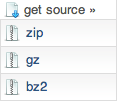
\includegraphics[scale=0.7]{Images/Bitbucket2.png}}
\caption{Téléchargement du code source (Bitbucket).}
\end{figure}

Ce mode de récupération est très simple mais présente un gros inconvénient : il sera impossible de mettre Galaxy à jour de cette façon.

\subsection*{Mercurial}

Mercurial est un outil de gestion de versions développé depuis 2005 sous licence GNU GPL. Principalement écrit en Python et utilisable en ligne de commande, Mercurial n'en est pas moins rapide, robuste et facile d'utilisation.\\

Toutes les commandes de Mercurial commencent par \textit{hg}, formule chimique du mercure.\\

La copie du répertoire distant tient en quelques commandes : 
\lstset{language=sh}
\begin{lstlisting} [morekeywords={mkdir,hg}]
mkdir Galaxy
cd Galaxy
hg clone https://bitbucket.org/galaxy/galaxy-dist/
 \end{lstlisting} 

Le clonage prend un certain temps. Mercurial doit en effet analyser les nouveautés du répertoire distant et télécharger les fichiers un par un. Le dossier final contient $\sim$8000 fichiers pour une taille totale d'environ 700 Mo.\\

L'intérêt d'utiliser Mercurial pour récupérer le code source est de pouvoir mettre ce code à jour, contrairement à Bitbucket.\\
La mise à jour utilise le système de modification distance de Mercurial. Elle tient donc en deux commandes\footnote{A exécuter dans le répertoire local de Galaxy} : 
\lstset{language=sh}
\begin{lstlisting} [morekeywords={hg}]
hg incoming
hg pull -u
 \end{lstlisting} 
 La première commande indique si des modifications ont été apportées. Si elle renvoie \textit{no changes found}, la version locale est à jour. Dans le cas contraire, elle renvoie une liste de \textit{changeset} (Fig. 10). La seconde commande peut être exécutée si au moins \textit{changset} est indiqué.

\begin{figure}[!h]
 \centering

\fbox{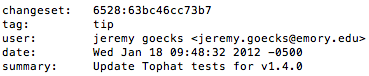
\includegraphics[scale=0.7]{Images/Changeset.png}}
\caption{Exemple de \textit{changeset} (Mercurial).}
\end{figure}

\subsection{Exécution du serveur local}

Galaxy fonctionne sur la base d'un serveur local. Cela consiste à ouvrir un serveur fictif sur l'ordinateur de l'utilisateur et à se servir de l'interface proposée par un navigateur web pour accéder aux services proposés par le serveur.\\

Ce logiciel étant principalement écrit en Python, il est officiellement compatible avec les versions 2.5, 2.6 et 2.7 de l'interpréteur Python par défaut. La version par défaut est donnée en en-tête de l'interpréteur  
(Fig. 11).

 \begin{figure}[!h]
 \centering
\fbox{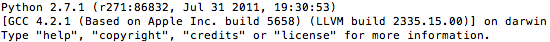
\includegraphics[scale=0.7]{Images/Python.png}}
\caption{Version de l'interpréteur Python.}
\end{figure}

Pour lancer le serveur local de Galaxy, il suffit d'exécuter le script \textit{run.sh} : 
\lstset{language=sh}
\begin{lstlisting} [morekeywords={sudo}]
sh run.sh # commande de base
sudo run.sh # commande administrateur
 \end{lstlisting} 
 
 La commande "de base" suffit à démarrer le serveur. Il est toutefois conseillé d'utiliser la commande administrateur car certaines opérations \footnote{Notamment l'écriture sur disque dur.} nécessitent des droits d'administrateur.\\
 
 Le serveur charge tous les fichiers requis, configure ses variables et démarre sur une adresse indiquée sur la dernière ligne du terminal (Fig. 12).
 
 \begin{figure}[!h]
 \centering
\fbox{
\includegraphics[scale=0.7]{Images/Adresselocale.png}}
\caption{Adresse du serveur de Galaxy.}
\end{figure}

Pour stopper le serveur, il suffit d'utiliser \textit{ctrl+z} dans le terminal qui le gère.\\

Il est possible que le port utilisé par Galaxy soit déjà en utilisation. Dans ce cas, le démarrage du serveur échoue et renvoie une erreur \textit{adress already in use} (Fig. 13). Seul un redémarrage de l'ordinateur peut réinitialiser le port.

 \begin{figure}[!h]
 \centering
\fbox{
\includegraphics[scale=0.7]{Images/Socketerror.png}}
\caption{Erreur d'adressage de port.}
\end{figure}
Une fois le serveur démarré, son accès est possible depuis un navigateur web quelconque (Fig. 14). L'adresse URL à indiquer est l'adresse donnée sur la dernière ligne du terminal.

 \begin{figure}[!h]
 \centering
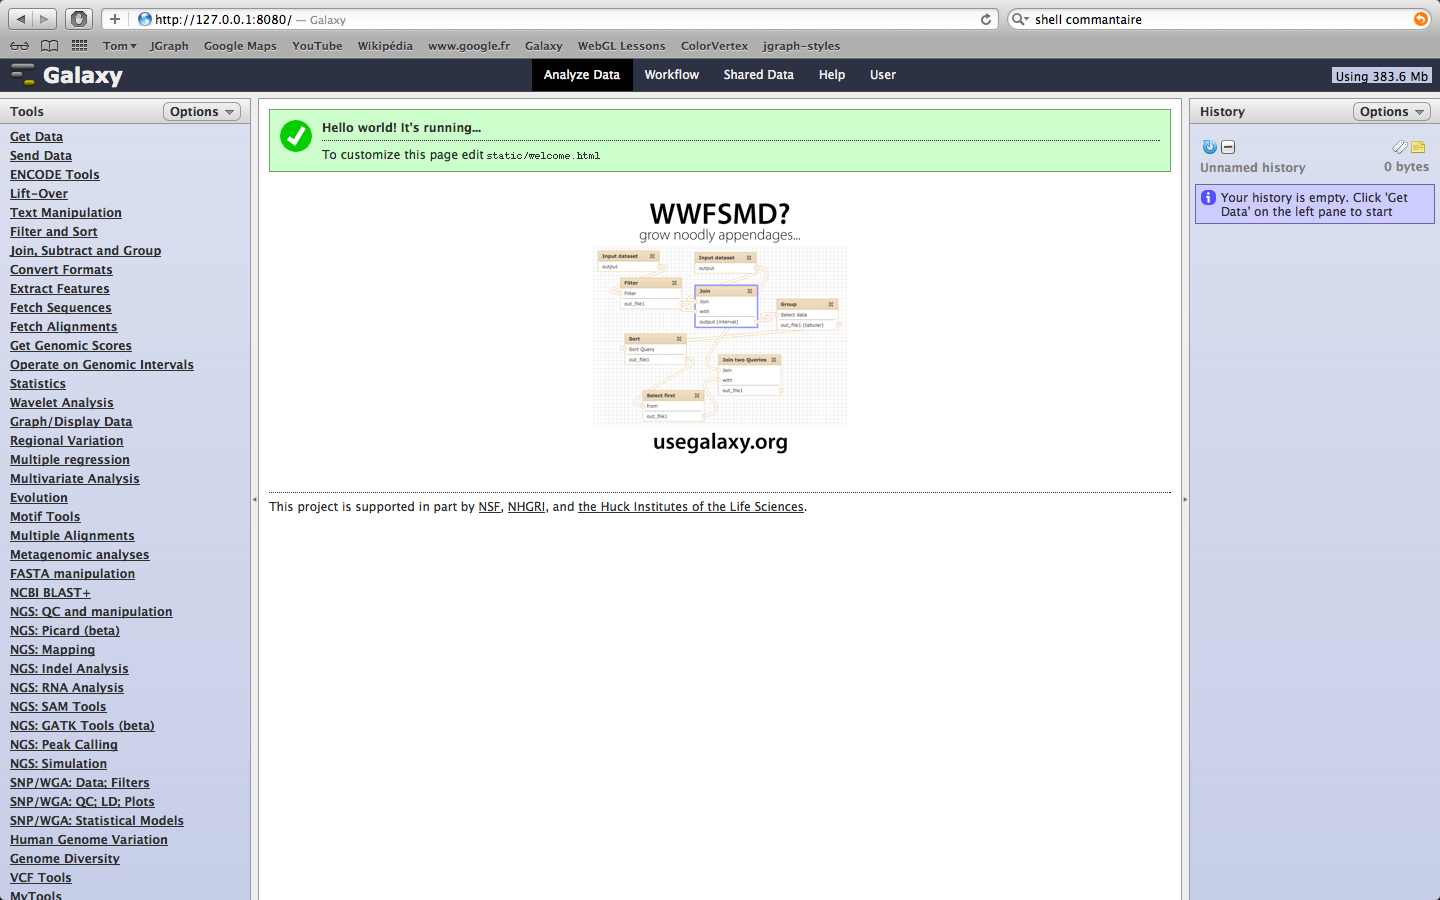
\includegraphics[scale=0.35]{Images/Galaxylocal.png}
\caption{Galaxy en usage local.}
\end{figure}
\chapter{Fonctionnalités}

Il nous est impossible de recenser et décrire toutes les fonctionnalités disponibles sous Galaxy. Nous nous limiterons donc la description des fonctionnalités aux principales ainsi qu'à l'ajout de plug-ins, permettant ainsi une personnalisation, ainsi que l'utilisation des workflows.

\section{Présentation générale}

Les outils de Galaxy peuvent être classés en quatre grande catégories.
\begin{enumerate}
\item Manipulation de fichiers :
	\begin{itemize}
	\item ouverture de fichiers volumineux,
	\item ajout/suppression de lignes,
	\item concaténation, filtrage, intersection,
	\item etc ...
	\end{itemize}
\item Opérations sur les données :
	\begin{itemize}
	\item addition, soustraction, moyenne, calcul de taille de séquences,
	\item conversion, formatage,
	\item etc ...
	\end{itemize}
\item Analyse de séquences :
	\begin{itemize}
	\item calcul de corrélation,
	\item recherche d'orthologues,
	\item utilisation des outils d'EMBOSS\footnote{European Molecular Biology Open Software Suite : suite logicielle dédiée aux analyses bioinformatiques},
	\item etc ...
	\end{itemize}
\item Visualisation des données :
	\begin{itemize}
	\item alignements multiples,
	\item distribution de données (histogramme, scatterplot),
	\item arbres phylogéniques,
	\item etc ...
	\end{itemize}
\end{enumerate}

\newpage
\section{Ajout de plug-ins}

L'ajout de plug-ins est une fonctionnalité uniquement disponible pour Galaxy installé localement. Pour implémenter une fonctionnalité, il faut commencer par développer le script/programme qui fera office de plug-in puis l'intégrer dans la liste des outils.

\subsection{Création}

Même si le cœur de Galaxy est dépendant Python, son architecture lui permet de gérer des scripts écrits dans différents langages de programmation interprétés\footnote{Tels que : Python, Ruby, Perl, Bash, etc ...} mais aussi compilés\footnote{Tels que : C, C++, Java, etc ...}. Cet avantage permet à (presque) tous les programmeurs de développer des outils dans leurs langages favoris, et de les intégrer en toute transparence dans Galaxy.\\

La communication Galaxy/fichiers est simple car fait intervenir les flux d'entrée/sortie en les redirigeant automatiquement vers :
\begin{itemize}
\item les fichiers intégrés dans Galaxy pour le flux d'entrée,
\item la fenêtre de résultats pour le flux de sortie.\\
\end{itemize}

Il n'est donc pas nécessaire de préparer une configuration spéciale puisque elle est réalisée par Galaxy.

\subsection{Intégration}

Afin de distinguer et de recenser tous les outils qui lui sont disponible, le logiciel possède une base de données de plug-ins sous la forme d'un fichier XML : \textit{tool\_conf.xml}.\\

\textit{tool\_conf.xml} agit en réalité comme une liste de pointeur : chaque plug-ins est identifié par un nom, un identifiant et un fichier XML qui correspond à un fichier de configuration. Pour faire savoir qu'un nouveau script est disponible, il suffit d'ajouter les lignes génériques :

\lstset{language=XML}
\begin{lstlisting} [morekeywords={section,tool}]
<section name="MyTools" id="mTools">
    <tool file="myTools/toolExample.xml" />
 </section>
 \end{lstlisting} 
 
Avec les attributs : 
\begin{itemize}
\item name : nom de l'outil tel qu'il apparaitra dans l'interface de Galaxy,
\item id : identifiant de l'outil,
\item file : chemin vers le fichier de configuration XML.\\
\end{itemize}

Il est conseillé, pour des raisons pratiques, de créer un répertoire contenant les scripts de l'utilisateur afin de les différencier des autres.\\ Dans l'exemple précédent, le futur plug-in ainsi que son fichier de configuration (\textit{toolExample.xml}) devront être placés dans un dossier \textit{tools/myTools} que l'utilisateur devra préalablement créer.\\

\newpage
\textit{toolExample.xml} doit au moins contenir les informations suivantes\footnote{Basé sur le tutorial : http://wiki.g2.bx.psu.edu/Admin/Tools/Add\%20Tool\%20Tutorial} : 

\lstset{language=XML}
\begin{lstlisting} [morekeywords={description,command,inputs,param,inputs,input,output,outputs,data,tests,test,help,tool}]
<tool id="fa_gc_content_1" name="Compute GC content">
  <description>for each sequence in a file</description>
  <command interpreter="perl">toolExample.pl $input $output</command>
  <inputs>
    <param format="fasta" name="input" type="data" label="Source file"/>
  </inputs>
  <outputs>
    <data format="tabular" name="output" />
  </outputs>

  <tests>
    <test>
      <param name="input" value="fa_gc_content_input.fa"/>
      <output name="out_file1" file="fa_gc_content_output.txt"/>
    </test>
  </tests>

  <help>
This tool computes GC content from a FASTA file.
  </help>
</tool>
 \end{lstlisting} 

Dans cet exemple, l'outil implémenté est un script Perl qui calcule le GC\%. Ce script prend 2 argument lors de son exécution : \$input (associé à un fichier interne au format fasta) et \$output (associé à la sortie standard de Galaxy : la fenêtre de résultats (Fig XX, XX et XX).\\




\begin{figure}[!h]
   \begin{minipage}[b]{0.40\linewidth}
      \centering 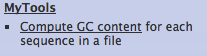
\includegraphics[scale=0.7]{Images/Ongletmytools.png}
      \caption{Onglet de l'outil implémenté.}
   \end{minipage}\hfill
   \begin{minipage}[b]{0.48\linewidth}   
      \centering 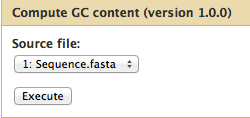
\includegraphics[scale=0.5]{Images/Gccontent.png}
      \caption{Fenêtre de l'outil implémenté.}
   \end{minipage}
\end{figure}

 \begin{figure}[!h]
 \centering
\fbox{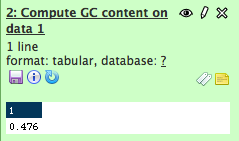
\includegraphics[scale=0.6]{Images/Resultatgc.png}}
\caption{Résultat du script \textit{toolExample.pl}.}
\end{figure}

Nous pouvons ainsi résumer les opérations nécessaires à l'intégration d'un plug-in de la façon suivante : 
\begin{enumerate}
\item écrire le script,
\item modifier \textit{tool\_conf.xml},
\item créer le fichier de configuration XML.
\end{enumerate}
\section{Workflow}

Le workflow Galaxy fournit un ensemble d’outils pour la manipulation et l’analyse de données génomiques. Il est très intuitif dans l’utilisation ce qui en fait une cible de choix pour le biologiste.\\


Il permet de créer des workflows, les enregistrer dans un espace dédié, les partager, et les exécuter de façon automatique. Les outils dédiés analyse de données NGS sont régulièrement mis à jour.\\


Galaxy offre donc la possibilité d’exécuter des analyses bioinformatiques sans effort de programmation. La version en ligne est intéressante car elle permet de se familiariser aux logiciels et d'exécuter l’analyse depuis un portable, mais la possibilité d’intégrer ces propres outils est indéniablement un gros avantage de la version locale.\\

Si nous devions citer un inconvénient, plutôt d’actualité : l’utilisateur est obligé de charger ses données en mémoire dans Galaxy, le temps de chargement peut être très long si l’on manipule des données issues d’expériences NGS, même sur une instance locale. Il est impensable de charger de telles données sur la version web.\\

Prenons par exemple un workflow de métagénomique (Fig. 18).\\

\begin{figure}[!h]
 \centering
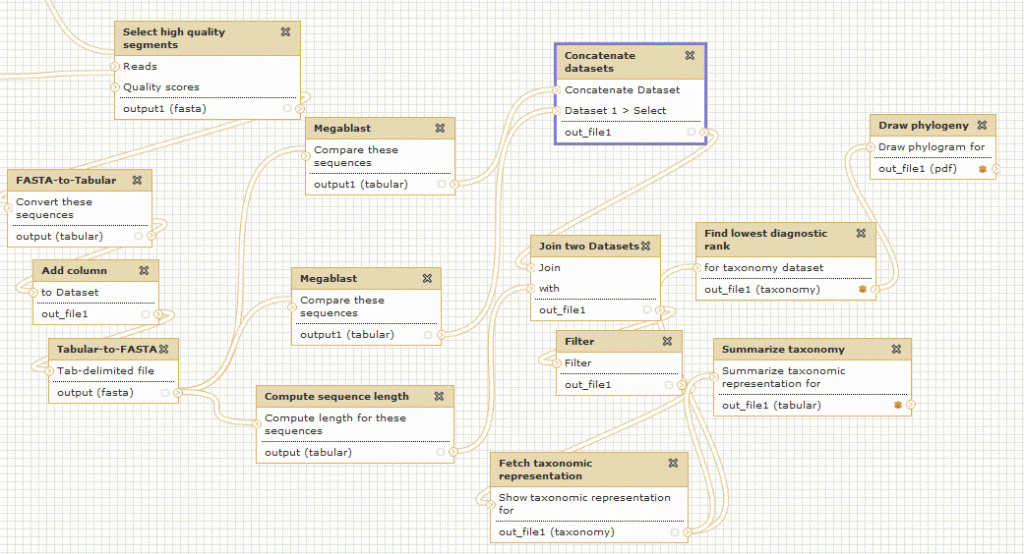
\includegraphics[scale=0.4]{Images/metagenomics.png}
\caption{Workflow de métagénomique.}
\end{figure}

La métagénomique étudie les organismes microbiens directement dans leur environnement sans passer par une étape de culture en laboratoire. Dans ce cas nous cherchons à obtenir des informations relatives à l'origine phylogénétique de l'organisme étudié et aussi des informations taxonomiques.\\
Pour cela, le workflow prend en entrée des fichiers issu de NGS 454. Dans la première entrée le workflow demande le fichier de read et la deuxième entrée celui de qualité.
\newpage

Ensuite, ces données passe par un programme chargé de sélectionner les segments de plus grande qualité. Ce programme à comme sortie un fichier au format FASTA.  Le principe ensuite est de lancer deux mégaBlast pour comparer les séquences à deux bases de données différentes. Mais pour cela il faut que chaque séquence "de qualité" soit identifiée donc on passe le fichir FASTA sortant du premier programme dans un convertisseur vers un format tabular, on rajoute une colonne qui content le numéro du read et on repasse au format FASTA.\\
 
En parallèle on lance un programme qui retourne un tableau avec dans la première colonne le nom de la séquence et dans la deuxième la longueur en acide nucléique. Les sorties des fichiers de blast sont mises dans un même fichier. Le tableau de longueur des séquences est lui aussi agrégé dans un autre programme. Le fichier sortant de ce programme passe dans un nouveau programme qui lui prépare les informations pour l'analyse taxonomique et l'analyse phylogénétique.\\

Donc la sortie de ce programme est envoyée à deux autres programmes un pour l'analyse phylogénétique et l'autre pour la finalisation de l'analyse taxonomique. Au final on obtient un fichier au format PDF avec l'arbre phylogénétique et un fichier comportant toute les informations taxonomiques.\\



Ce qui est agréable dans un tel type de workflow est la simplicité de mise en place, surtout avec l'interface graphique ou les programme sont représenté par des boites relié entre elles part des flèches. Ces flèches correspondent aux fichiers qui vont d'une application à un autre.\\
\chapter*{Conclusion}
\addcontentsline{toc}{chapter}{Conclusion}

Les logiciels de Workflow tel Galaxy s’inscrivent dans une logique de pérennisation des processus analytiques, qui a pour but de sortir de la logique « projet » (dans le sens ponctuel) en créant des processus d’analyses génériques. Comme nous l'avons vu, un logiciel de Workflow est un outil permettant d’exécuter un ensemble de processus de façon automatique. Ces « pipelines » sont très présents en bioinformatique (à défaut d’être tres utilisés) car ils permettent aux chercheurs en biologie d’analyser leurs données (issues de séquencages, génotypages) de façon relativement transparente et (quasiment) sans l’aide d’informaticiens (denrées rares dans la recherche).

Toutefois, il conviendra de distinguer deux sortes de logiciel de Workflow :
\begin{itemize}
\item{Les logiciels de Workflow qui permettent aux chercheurs de manipuler leurs données et exécuter leurs analyses sans posséder de connaissances en écriture de scripts ou en bases de données. Les données sont rapatriées au sein du logiciel de Workflow, permettant l’exécution d’un ensemble de tâches, à travers des modules pré-installés. En séquençage, le Workflow permet de convertir des séquences en formats divers, les filtrer  ou les assembler .Le logiciel de Workflow ISYS (2001), BioMOBY, Taverna et Galaxy entrent dans cette catégorie.}

\item{Les logiciels de Workflow qui assurent un accès direct à des composants (installés sur le serveur) et/ou aux données génomiques sans passer par un rapatriement préalable des données. WildFire, Pegasys ou Ergatis (ce dernier sera décrit dans un prochain post) font partie de cette catégorie. De manière générale ces logiciels de Workflow sont plus difficiles à prendre en main mais sont évidemment plus flexibles.}
\end{itemize}
Pour résumer, Galaxy permet :
\begin{itemize}
\item{D’automatiser des processus d’analyse (idéalement répétitifs) en les reliant dans un pipeline}
\item{De lancer des analyses sur des architectures matérielles complexes telles des grilles de calculs ou des serveurs}
\item{ De formaliser le processus d’analyse en vue d’une publication scientifique}
\end{itemize}

%%%%%%%%%%%%%%%%%%%%%%%%%%%%%%%%%%%%%%%%%%%%%%
%% Gestion et insertion de la bibliographie %%
%%%%%%%%%%%%%%%%%%%%%%%%%%%%%%%%%%%%%%%%%%%%%%

% le fichier a modifier est bibl/biblio.bib.
% On peut le remplir a la mano ou
% sinon il existe des prog plus conviviale.
% Google is your friends ^^

\bibliographystyle{plain}	% (uses file "plain.bst")
\bibliography{Reference}		% expects file "myrefs.bib"
\nocite{*}
\label{sec:bibli}
%%%%%%%%%%%%%%%%%%%%%%%%%%%%%%%%%%%%%%%%%%%%%%

%%%%%%%%%%%%%%%%%%%%%%%%%%%%%%%%%%%%%%
%% Gestion et insertion des annexes %%
%%%%%%%%%%%%%%%%%%%%%%%%%%%%%%%%%%%%%%

%\appendix
%\appendixpage
%\addappheadtotoc
%\renewcommand{\thesection}{\Alph{section}.}

\end{document}


